\chapter{Test}
\label{7-test}

To test the application I used Cucumber with user stories for acceptance tests with Zombie as a headless browser and Istanbul for code coverage testing. I also used a mock server to get mock data during testing, because the back end modules are not finished yet.

\section{Communication Interfaces}
As I mentioned in \refstruc{api-blueprint}, I used the API Blueprint specification to define the communication interfaces. 

\emph{Example GET:}

\# Message {[}/student/\string{userid\string}/general{]}\\
\#\# Get student general informations [GET]\\
$+$ Response 200 (application/json)
\begin{addmargin}[1em]{1em}
	\string{
	\begin{addmargin}[1em]{1em}
		"name" : "Teszt Hallgató",\\
		"neptun" : "Neptun",\\
		"id" : "1"
	\end{addmargin}
	\string}
\end{addmargin}

This example sends the same json response for every HTTP GET request. The \emph{userid} is a wildcard parameter, the server will send the same response. I used the parameter \emph{1} for testing.
	
	
\emph{Example POST}:

\# Message {[}/student/\string{userid\string}/setsettings{]}\\
\#\#\# Post new settings for student {[}POST{]}\\
\#\# Automatic response to OPTIONS requests

+ Request (application/json)
\begin{addmargin}[1em]{1em}
	+ Schema
		\begin{addmargin}[1em]{1em}
		\string{   "type":"object",
			\begin{addmargin}[1em]{1em}
				"required": {[}"notification", "mailingList"{]},\\
				"properties" : \string{
					\begin{addmargin}[1em]{1em}
						"email": \string{"type":"string"\string},\\
						"notification": \string{"type":"boolean"\string},\\
						"mailingList": \string{"type":"boolean"\string},\\
						"sshPublicKey": \string{"type":"string"\string},\\
						"oldpwd": \string{"type":"string"\string},\\
						"newpwd": \string{"type":"string"\string}
					\end{addmargin}
				\string}
			\end{addmargin}
		\string}
		\end{addmargin}
\end{addmargin}

+ Response 201 (application/json;charset=UTF-8)
\begin{addmargin}[1em]{1em}
	+ Body
	\begin{addmargin}[1em]{1em}
		\string{
			\begin{addmargin}[1em]{1em}
				status": "ok"
			\end{addmargin}
			\string}
	\end{addmargin}
\end{addmargin}
	
This example sends the same json response for every HTTP POST or OPTIONS request, where the body matches the JSON Schema. Only two parameters are required, but the body cannot contain any parameter, that is not defined in the properties section.

The API blueprint files are available on Github.\todo{link} Mock server usage is described in \refstruc{mock-server-usage}.


\section{Testing}
The following features were implemented:

\begin{enumerate}
	\item see the general information about the classes
	\setcounter{enumi}{0}
	\item see the results
	\item see a list of commits and tagging a commit as final version
	\setcounter{enumi}{1}
	\item set new password, e-mail and SSH public key
	\item summarized view of student's grades
\end{enumerate}

As I mentioned in \refstruc{design-specification}, I tested the features with priority levels 1 and 2.

\subsection{Acceptance Tests}
An acceptance test validates that this is the software or feature the customer wanted. I wrote user stories \see{spec-user-story} for the features I wanted to test based on the user stories I wrote during the specification phase. 

During the testing I was comparing the HTML element's existence and compared the included texts with the example data that came form the user story. If a label contains a date, I used a regex for pattern matching:

\monospace{(\textbackslash d{4})\textbackslash.(\textbackslash d{2})\textbackslash.(\textbackslash d{2})\textbackslash. (\textbackslash d{2}):(\textbackslash d{2})}

Because I cannot test features, that needs to change the database, without a real back end, I tested for requests. If there was an outgoing request for the specific URL, the test passed. These tests will change when the back end modules will be implemented.

\subsubsection{Cucumber}
\label{cucumber-test}

I used Cucumber \see{spec-cucumber} to implement acceptance tests. I used the instructions on the Cucumber website to start the implementation~\cite{github-cucumberjs}. A Cucumber test requires the following files:

\begin{itemize}
	\item \textbf{Features Files:} The user stories are stored in feature files.
	\item \textbf{Support Files:} These will be run before each scenario to create the test environment. In my case it creates a headless browser. One example is included on the Cucumber website, but that does not work. I implemented my own support file.
	\item \textbf{Step Definitions:} These are the implemented feature steps. I generated the functions with a JetBrains plugin~\cite{jetbrains-cucumber} and implemented the logic for every step. 
\end{itemize}

\subsubsection{Zombie}
I wanted to use a browser to test the client's JavaScript code. My first choice was Selenium~\cite{selenium} with a Google Chrome browser, but the tests were slow. To solve this issue I have decided to use a browser without a user interface. I chose Zombie, because it was recommended on the Cucumber website.

Zombie~\cite{zombie} is lightweight framework, that implements a browser without a user interface. It also supports assertions, that makes it possible to text field comparison and HTML element existence testing easier, and pipelines to log the outgoing requests from the Zombie browser. 

\subsection{Code Coverage Tests}

\subsubsection{Istanbul}
Istanbul~\cite{istanbul} is a code coverage software tool for JavaScript. It checks coverage for:

\begin{itemize}
	\item \emph{Function:} number of functions, that have been called.
	\item \emph{Statement:} number of statements, that have been executed.
	\item \emph{Branch:} Number of branches, that have been executed.
\end{itemize}

\subsection{Automatized Tests}
First follow the instructions in \refstruc{deployment}, then start the mock server. Use the following command to run the Cucumber tests:

\monospace{npm test}

Use the following command to run the Cucumber tests with code coverage:

\monospace{npm test \texttt{-{}-}coverage}

I have implemented 14 scenarios and 91 steps.

\subsubsection{Test Results}

\begin{figure}[!ht]
	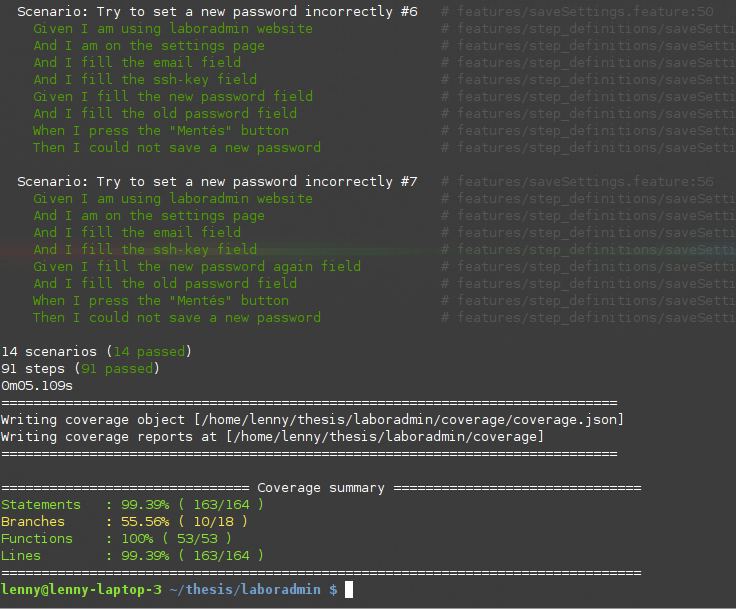
\includegraphics[width=\textwidth]{figures/test-result.png}
	\caption{Test Results}
	\label{fig:test-results}
	\end{figure}

